\chapter{Results}

\section{Case Study: Heart Failure}

\subsection{Peak-value Clustering}

\begin{figure}[h!]
    \begin{center}
    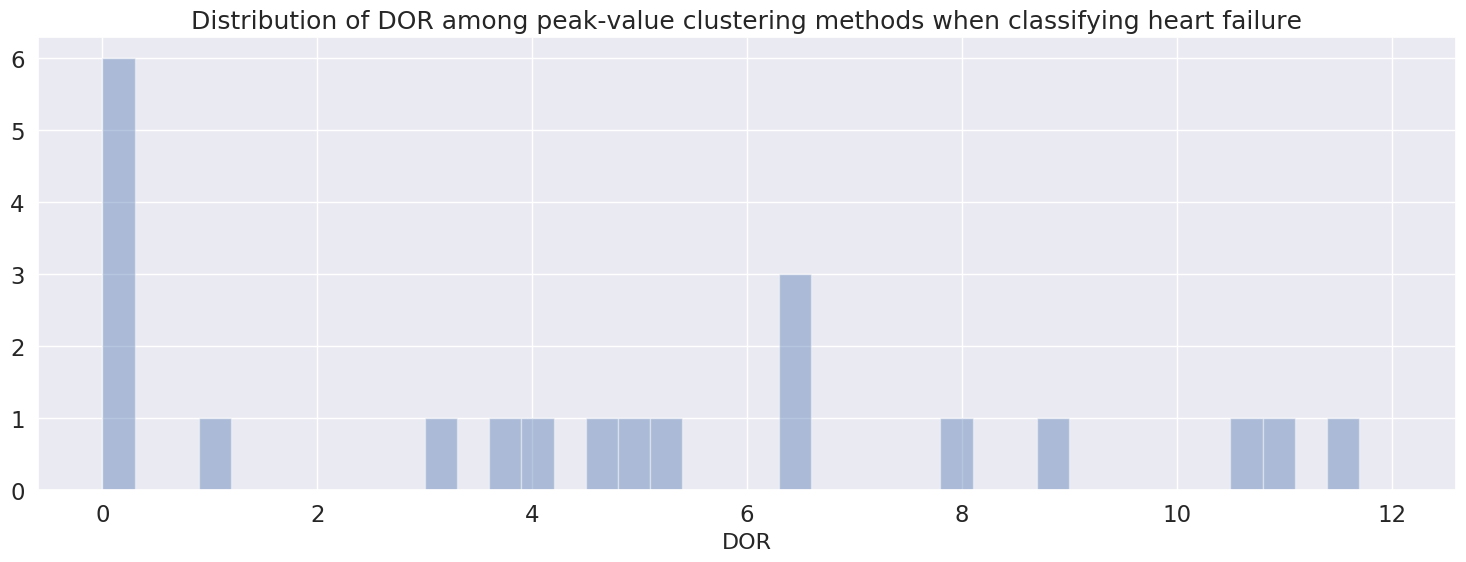
\includegraphics[width=\textwidth]{results/pvc-hf-dor.png}
    \end{center}
    \caption{DOR distribution of PVC methods when classifying heart failure.}
    \label{fig:pvc_hf_dor}
\end{figure}

\begin{figure}[!h]
    \begin{center}
    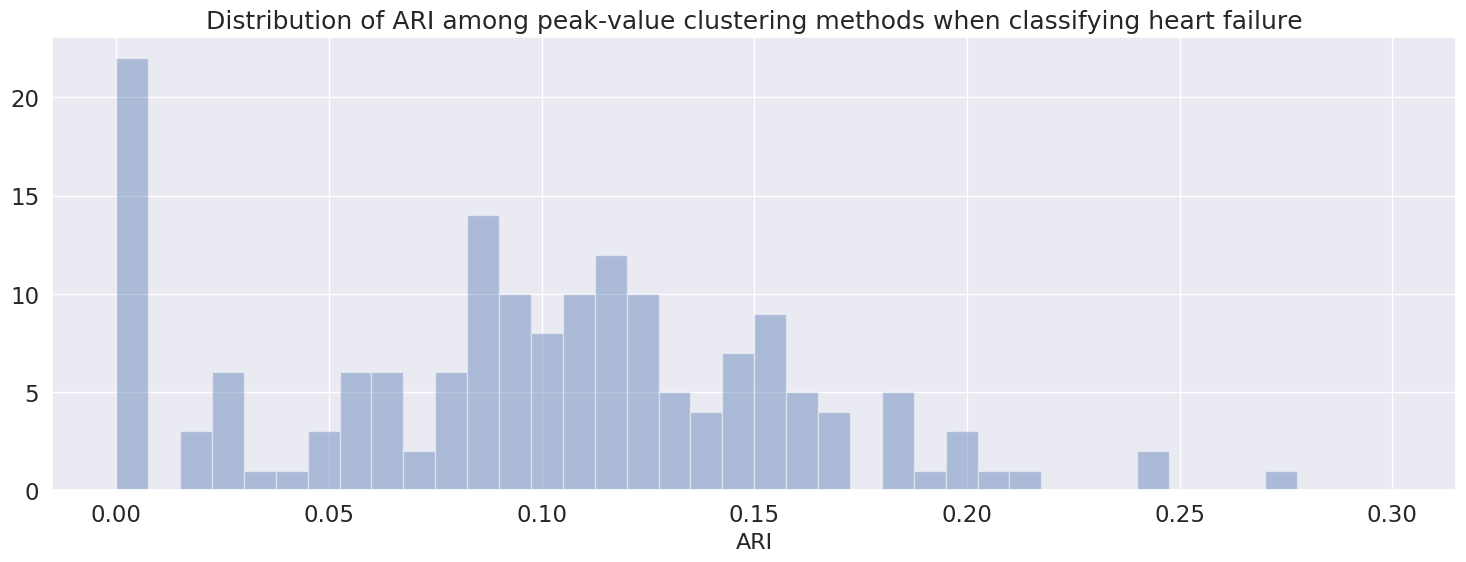
\includegraphics[width=\textwidth]{results/pvc-hf-ari.png}
    \end{center}
    \caption{ARI distribution of PVC methods when classifying heart failure.}
    \label{fig:pvc_hf_ari}
\end{figure}

\subsection{Time-series Clustering}

\begin{figure}[h!]
    \begin{center}
    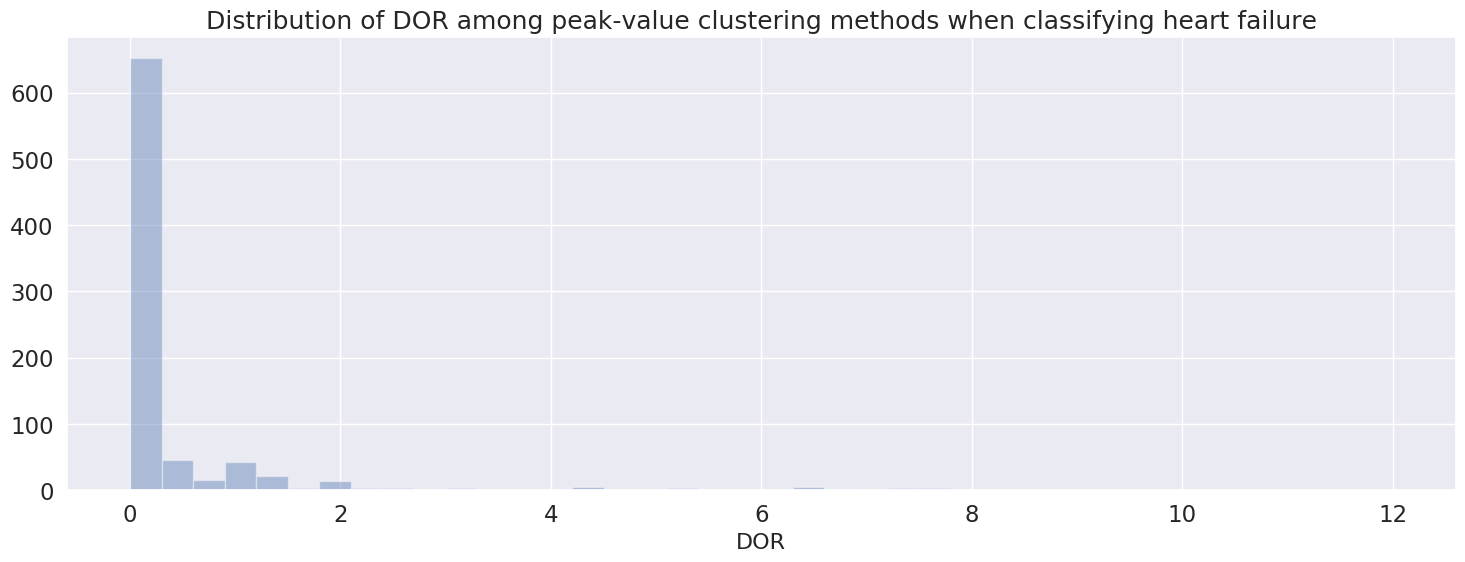
\includegraphics[width=\textwidth]{results/tsc-hf-dor.png}
    \end{center}
    \caption{DOR distribution of TSC methods when classifying heart failure.}
    \label{fig:}
\end{figure}

\begin{figure}[h!]
    \begin{center}
    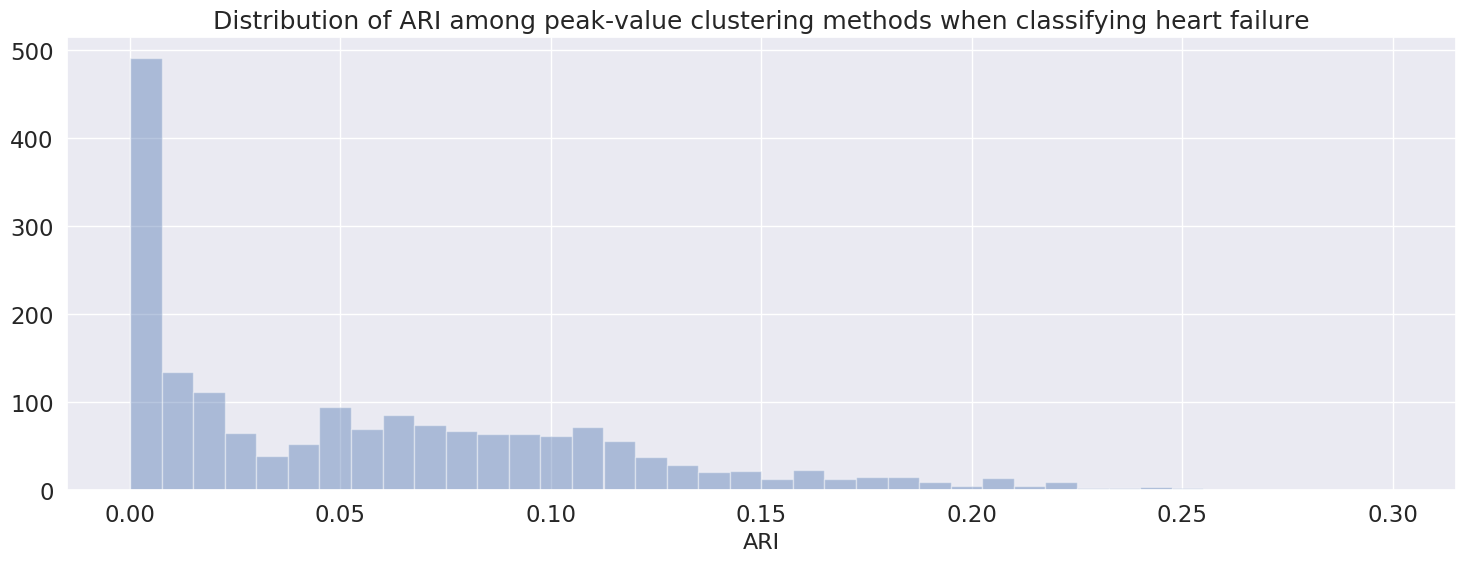
\includegraphics[width=\textwidth]{results/tsc-hf-ari.png}
    \end{center}
    \caption{ARI distribution of TSC methods when classifying heart failure.}
    \label{fig:}
\end{figure}

\subsection{Deep Neural Network}

% \begin{figure}[h!]
%     \begin{center}
%     \includegraphics[width=\textwidth]{results/}
%     \end{center}
%     \caption{.}
%     \label{fig:}
% \end{figure}

\subsection{Peak-value Classifiers}

% \begin{figure}[h!]
%     \begin{center}
%     \includegraphics[width=\textwidth]{results/}
%     \end{center}
%     \caption{.}
%     \label{fig:}
% \end{figure}

\subsection{Comparisons}

\newpage

\section{Case Study: Patient Diagnosis}

\subsection{Peak-value Clustering}

\begin{figure}[h!]
    \begin{center}
    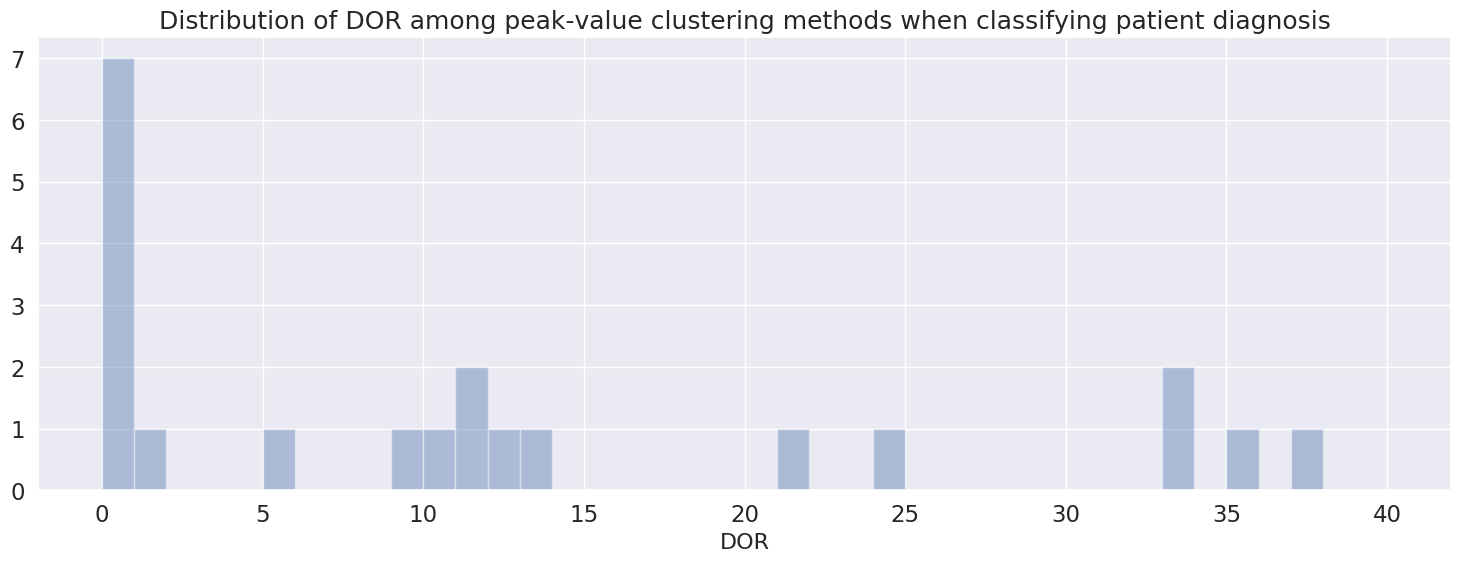
\includegraphics[width=\textwidth]{results/pvc-ind-dor.png}
    \end{center}
    \caption{DOR distribution of PVC methods when classifying patient diagnoses.}
    \label{fig:pvc_ind_dor}
\end{figure}

\begin{figure}[h!]
    \begin{center}
    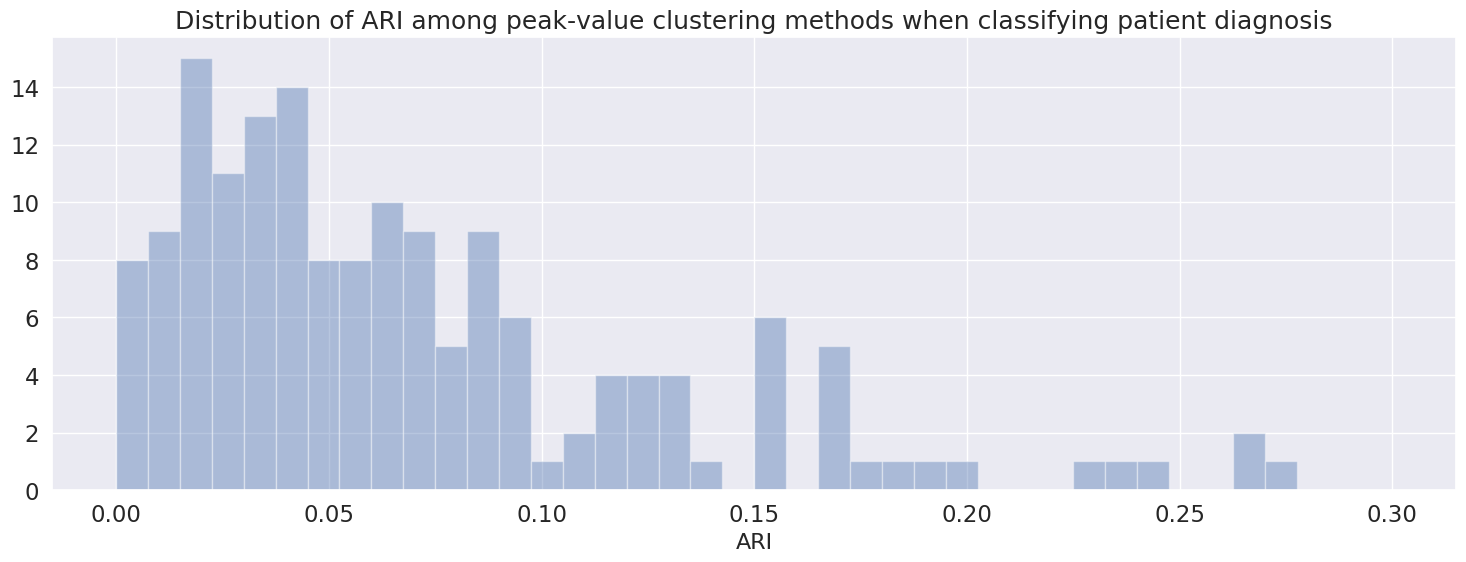
\includegraphics[width=\textwidth]{results/pvc-ind-ari.png}
    \end{center}
    \caption{ARI distribution of PVC methods when classifying patient diagnoses.}
    \label{fig:pvc_ind_ari}
\end{figure}

\subsection{Time-series Clustering}

\begin{figure}[h!]
    \begin{center}
    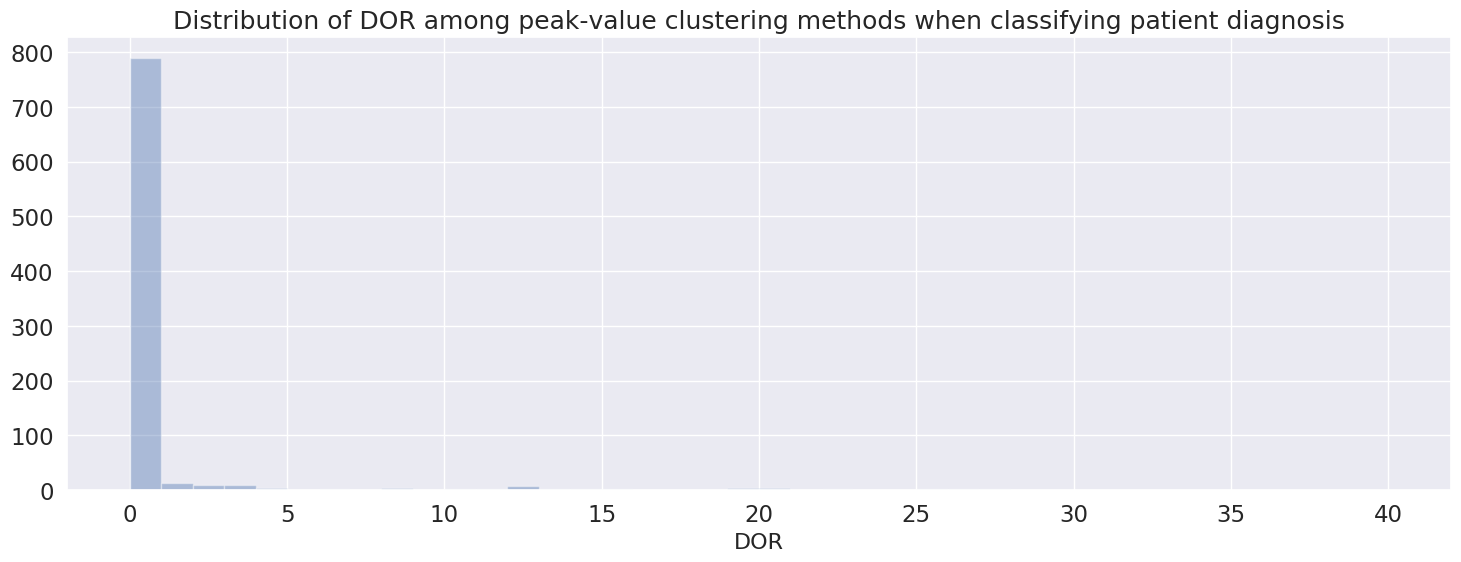
\includegraphics[width=\textwidth]{results/tsc-ind-dor.png}
    \end{center}
    \caption{DOR distribution of TSC methods when classifying patient diagnoses.}
    \label{fig:tsc_ind_dor}
\end{figure}

\begin{figure}[h!]
    \begin{center}
    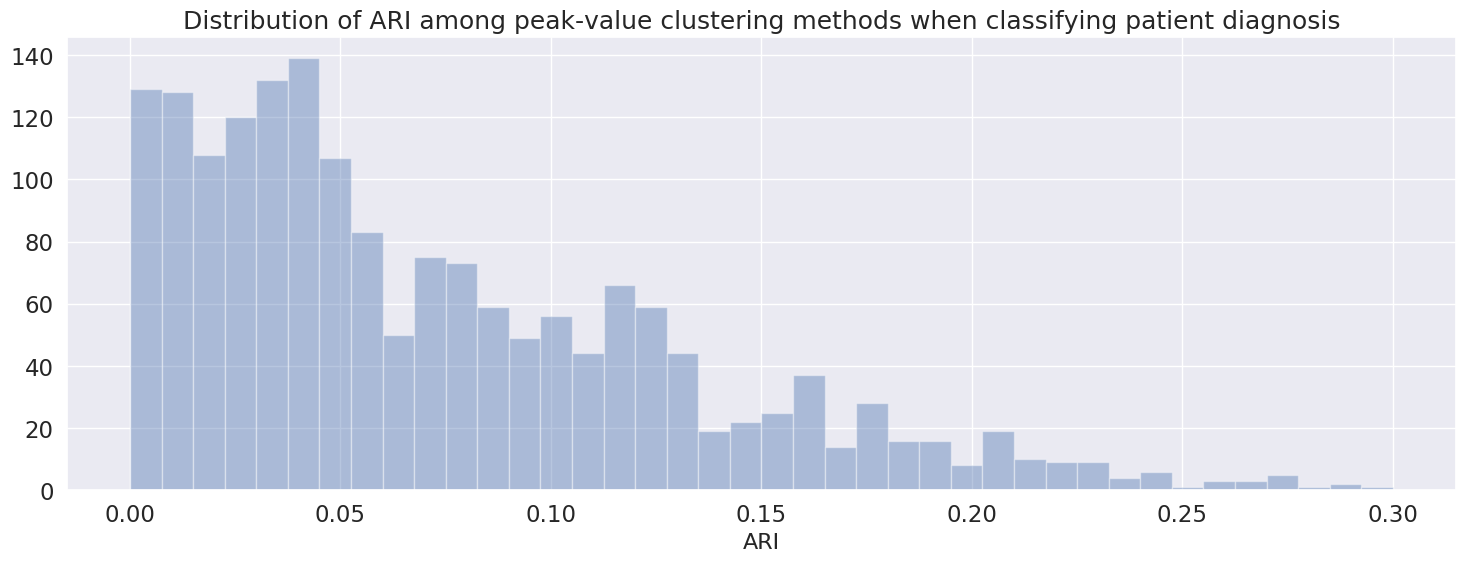
\includegraphics[width=\textwidth]{results/tsc-ind-ari.png}
    \end{center}
    \caption{ARI distribution of TSC methods when classifying patient diagnoses.}
    \label{fig:tsc_ind_ari}
\end{figure}

\subsection{Deep Neural Network}

% \begin{figure}[h!]
%     \begin{center}
%     \includegraphics[width=\textwidth]{results/}
%     \end{center}
%     \caption{.}
%     \label{fig:}
% \end{figure}

\subsection{Peak-value Classifiers}

% \begin{figure}[h!]
%     \begin{center}
%     \includegraphics[width=\textwidth]{results/}
%     \end{center}
%     \caption{.}
%     \label{fig:}
% \end{figure}

\subsection{Comparisons}

\newpage

\section{Case Study: Segment Indication}

\subsection{Time-series Clustering}

% \begin{figure}[h!]
%     \begin{center}
%     \includegraphics[width=\textwidth]{results/}
%     \end{center}
%     \caption{.}
%     \label{fig:}
% \end{figure}

% \begin{figure}[h!]
%     \begin{center}
%     \includegraphics[width=\textwidth]{results/}
%     \end{center}
%     \caption{.}
%     \label{fig:}
% \end{figure}

\subsection{Deep Neural Network}

% \begin{figure}[h!]
%     \begin{center}
%     \includegraphics[width=\textwidth]{results/}
%     \end{center}
%     \caption{.}
%     \label{fig:}
% \end{figure}

\subsection{Peak-value Classifiers}

% \begin{figure}[h!]
%     \begin{center}
%     \includegraphics[width=\textwidth]{results/}
%     \end{center}
%     \caption{.}
%     \label{fig:}
% \end{figure}

\subsection{Comparisons}

\section{Chapter Summary}
